\subsection{adjoint functors}

\begin{frame}
Let $\mathcal{C}$, $\mathcal{D}$ be categories.
Let $F : \mathcal{C} \to \mathcal{D}$ and
$G : \mathcal{D} \to \mathcal{C}$ be functors.
We say that $F$ is a {\it left adjoint} of $G$ or that
$G$ is a {\it right adjoint} to $F$, written $F \dashv G$, if there are bijections
\begin{block}{Hom-set formulation of adjunction}
$$
\phi_{c,d}:\Mor_\mathcal{D}(Fc, d)
\simeq
\Mor_\mathcal{C}(c, Gd)
$$
\end{block}
functorial in $c \in \Ob(\mathcal{C})$, and
$d \in \Ob(\mathcal{D})$.
\end{frame}
%
\begin{frame}
Morphisms that are associated with each other according to the bijections of an adjunction are called {\it adjoint transposes} of one another. 

There is a correspondence
\begin{block}{}
\abovedisplayskip=0pt
\begin{align*}
g &: Fc \rightarrow d, \,\, g \in \Mor(\mathcal{D})\\
g^* &: c \rightarrow Gd, \,\, g^* \in \Mor(\mathcal{C})
\end{align*}
\end{block}
given by $\phi_{c,d}(g) = g^*$. 
Similarly for 
\begin{block}{}
\abovedisplayskip=0pt
\begin{align*}
f &: c \rightarrow Gd, \,\, f \in \Mor(\mathcal{C})\\
f^* &: Fc \rightarrow d, \,\, f^* \in \Mor(\mathcal{D}) 
\end{align*}
\end{block}
given by $\phi_{c,d}^{-1}(f) = f^*$. 
We see then that $g^* = f$ and $f^* = g$.
\end{frame}
%
\begin{frame}
Consider the identity morphism $1_{Fc} \in \Mor_{\mathcal{D}}(Fc,Fc)$. The adjoint transpose of $1_{Fc}$ is the {\it unit} morphism at $c$
\begin{block}{unit morphism}
\abovedisplayskip=0pt
$$
\phi_{c,Fc}(1_{Fc})=1_{Fc}^*=\eta_c: c \rightarrow GFc
$$
\end{block}
where $\eta_c \in \Mor_{\mathcal{C}}(c,GFc)$, which, when taken to be natural in $c \in \Ob(\mathcal{C})$, gives the natural transformation
\begin{block}{unit natural transformation}
\abovedisplayskip=0pt
$$
\eta : 1_{\mathcal{C}} \Rightarrow GF
$$
\end{block}
\end{frame}
%
\begin{frame}
Consider the identity morphism $1_{Gd} \in \Mor_{\mathcal{C}}(Gd,Gd)$. The adjoint transpose of $1_{Gd}$ is the {\it counit} morphism at $d$
\begin{block}{counit morphism}
\abovedisplayskip=0pt
$$
\phi_{Gd,d}^{-1}(1_{Gd})=1_{Gd}^*=\epsilon_d: FGd \rightarrow d
$$
\end{block}
where $\epsilon_d \in \Mor_{\mathcal{D}}(d,FGd)$, which, when natural in $d$, gives the natural transformation
\begin{block}{counit natural transformation}
\abovedisplayskip=0pt
$$
\epsilon: FG \Rightarrow 1_{\mathcal{D}}
$$
\end{block}
\end{frame}

\begin{frame}[t]
We can then give an alternative definition of adjoint functors in terms of the unit natural transformation (dually the counit natural transformation) as
\begin{align*}
F & \colon \mathcal{C} \rightleftarrows \mathcal{D} \colon G\\
\eta & \colon 1_{\mathcal{C}} \rightarrow GF
\end{align*}
where for any $c \in \Ob (\mathcal{C})$, $d \in \Ob (\mathcal{D})$, and $f \colon c \rightarrow Gd \in \Mor(\mathcal{C})$ there exists a unique $g \colon Fc \rightarrow d \in \Mor(\mathcal{D})$ such that $f = Gg \circ \eta_c$				
\begin{columns}[t]
    \begin{column}{0.5\textwidth}
     \begin{block}{unit conditions for $F \dashv G$}
		\abovedisplayskip=0pt
		$$
					\xymatrix{
					c \ar[r]^{\eta_c} \ar[dr]_{f} & G F c \ar[d]^{G g} & F c \ar@{.>}[d]^{g}\\
					& G d & d}
		$$
		\end{block}
    \end{column}
    \begin{column}{0.5\textwidth}
		     \begin{block}{adjoint correspondence}
		\abovedisplayskip=0pt
		$$
			\frac{c \longrightarrow Gd}{Fc \longrightarrow d}
		$$
		\end{block}
    \end{column}
\end{columns}
\end{frame}

\begin{frame}
We can then give an alternative definition of adjoint functors in terms of the counit natural transformation (dually the unit natural transformation) as
$$
F \colon \mathcal{C} \rightleftarrows \mathcal{D} \colon G
$$
$$
\epsilon \colon FG \rightarrow 1_{\mathcal{C}}
$$
where for any $c \in \Ob (\mathcal{C})$, $d \in \Ob (\mathcal{D})$, and $g \colon Fc \rightarrow d \in \Mor(\mathcal{D})$ there exists a unique $f \colon c \rightarrow Gd \in \Mor(\mathcal{C})$ such that $g = \epsilon_D \circ Ff$	
\begin{columns}[t]
    \begin{column}{0.5\textwidth}
\begin{block}{counit conditions for $F \dashv G$}
$$
			\xymatrix{
			& F c \ar[d]^{F f} \ar[dl]_{g} & c \ar@{.>}[d]^{f}\\
			d & F G d \ar[l]^{\epsilon_d} & G d}
$$
\end{block}
    \end{column}
    \begin{column}{0.5\textwidth}
		\begin{block}{adjoint correspondence}
		\abovedisplayskip=0pt
		$$
			\frac{Fc \longrightarrow d}{c \longrightarrow Gd}
		$$
		\end{block}
    \end{column}
\end{columns}
\end{frame}

\subsection{encoding and decoding}

\begin{frame}
The adjoint relationship between functors $F \dashv G$ with unit $\eta$ and counit $\epsilon$ natural transformations. The asymmetry in the encoding-decoding relationship indicates that $FG \mathcal{D}$ can be translated back into the original terms of $\mathcal{D}$ whereas $GF \cC^{opp}$ cannot necessarily be translated back into the original terms of $\cC^{opp}$.
\begin{center}
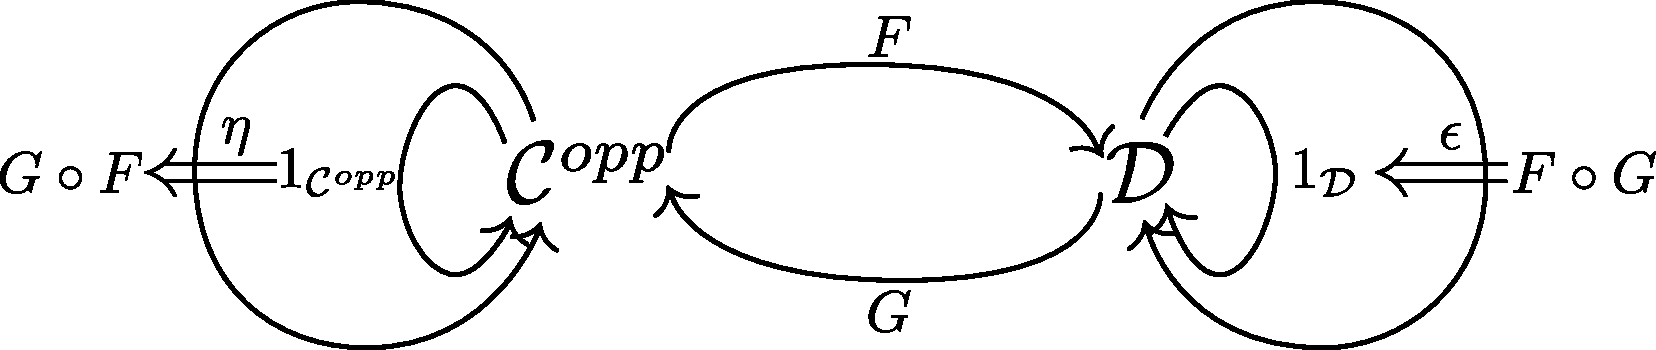
\includegraphics[width=0.9\framewidth]{fig/adjunction.pdf}
\end{center}
\end{frame}

\begin{frame}
The asymmetry of the adjunction can be dispensed with if the unit and counit natural transformations are in fact natural isomorphisms $\eta: 1_{\cC^{opp}} \cong GF$ and $\epsilon: FG \cong 1_{\mcD}$. In any limit in which this is the case the adjunction $F \dashv G$ gives an equivalence of categories $\cC^{opp} = \mcD$ and the information encoding-decoding process becomes bidirectionally exact.
\end{frame}

\subsection{Hom-tensor adjunction}
\begin{frame}[t]
\frametitle{$\times \dashv Hom$ adjunction}
\begin{block}{}
\abovedisplayskip=0pt
\begin{align*}
- \times Z: \mathcal{C} & \rightleftarrows \mathcal{C}: (-)^Z\\
\Mor_{\mathcal{C}}(X \times Z, Y) & \cong  \Mor_{\mathcal{C}}(X, Y^Z)
\end{align*}
\end{block}
\begin{block}{change notation}
	\begin{center}
	Let $\Pi_Z = - \times Z$ and $E^Z = (-)^Z$
	\end{center}
\end{block}
\begin{columns}[t]
    \begin{column}{0.5\textwidth}
		\begin{block}{functors on components}
			$$
			\xymatrix{
			& \Pi_Z X \ar[d]^{\Pi_Z \bar{f}} \ar[dl]_{f} & X \ar@{.>}[d]^{\bar{f}}\\
			Y & \Pi_Z E_Z Y \ar[l]^{\epsilon_Y} & E_Z Y}
			$$
		\end{block}		
    \end{column}
    \begin{column}{0.5\textwidth}
		\begin{block}{in components}
			$$
			\xymatrix{
			& X \times Z \ar[d]^{\bar{f} \times 1_Z} \ar[dl]_{f} & X \ar@{.>}[d]^{\bar{f}}\\
			Y & Y^Z \times Z \ar[l]^{\epsilon_Y} & Y^Z}
			$$
		\end{block}
    \end{column}
\end{columns}
\end{frame}

\begin{frame}[t]
\frametitle{$\times \dashv Hom$ adjunction}
\begin{block}{}
\abovedisplayskip=0pt
\begin{align*}
- \times Z: \mathcal{C} & \rightleftarrows \mathcal{C}: (-)^Z\\
\Mor_{\mathcal{C}}(X \times Z, Y) & \cong  \Mor_{\mathcal{C}}(X, Y^Z)
\end{align*}
\end{block}
\begin{block}{change notation}
	\begin{center}
	Let $\Pi_Z = - \times Z$ and $E^Z = (-)^Z$
	\end{center}
\end{block}
\begin{columns}[t]
    \begin{column}{0.5\textwidth}
\begin{block}{in components}
			$$
			\xymatrix{
			& X \times Z \ar[d]^{\bar{f} \times 1_Z} \ar[dl]_{f} & X \ar@{.>}[d]^{\bar{f}}\\
			Y & Y^Z \times Z \ar[l]^{\epsilon_Y} & Y^Z}
			$$
		\end{block}
    \end{column}
    \begin{column}{0.5\textwidth}
		\begin{block}{adjoint correspondence}
		\abovedisplayskip=0pt
		$$
			\frac{X \times Z \longrightarrow Y}{X \longrightarrow Y^Z}
		$$
		the counit is the evaluation map
		$$
			\epsilon_Y = ev_Y \colon Y^Z \times Z \longrightarrow Y
		$$
		\end{block}		
    \end{column}
\end{columns}
\end{frame}